% Chapter 3

\chapter{Évaluation et Feedback humain} 
\label{ch:3}

Bien que les \acp{llm} soient capables de restituer l'information avec une précision impressionnante, ils ne sont pas exempts d'erreurs et peuvent parfois produire des résultats erronés sous forme d'« hallucinations » \cite{zhu2024understanding, bai2024hallucination}. Ce terme désigne les instances où les modèles génèrent des contenus qui semblent plausibles mais qui ne sont pas fondés sur des faits réels ou vérifiables. Ces hallucinations peuvent inclure la fabrication de détails fictifs, la distorsion des informations existantes, ou l'émission de conclusions inexactes. Ce phénomène est particulièrement problématique dans le domaine juridique où la fiabilité et la précision des informations sont cruciales.

Étant donné notre objectif de vulgariser le Droit congolais de manière accessible et précise, il est impératif d'intégrer une couche d'évaluation humaine. Cette évaluation sera assurée par des professionnels du droit congolais, qui apporteront leur expertise pour vérifier et corriger les outputs du modèle. Leur rôle sera d'assurer que les informations générées par le chatbot soient non seulement correctes mais aussi pertinentes et utiles pour les utilisateurs finaux. Cette démarche permettra de pallier les limitations des \acp{llm} et de garantir que les informations diffusées respectent les normes juridiques et éthiques, renforçant ainsi la fiabilité et la crédibilité de notre projet.

L'intégration de feedback humain dans le processus d'évaluation contribue également à un cycle d'amélioration continue du modèle, où les corrections et les insights fournis par les experts peuvent être utilisés pour affiner et ajuster les algorithmes sous-jacents. Cette collaboration entre IA et expertise humaine est essentielle pour créer un outil robuste et fiable, capable de servir efficacement les besoins d'information juridique de la communauté.

\section{Critères et méthodes d'évaluations}

Dans une première phase d'évaluation, nous mettrons à l'épreuve les modèles existants en utilisant le test de magistrature congolais de 2022. Pour ce faire, nous appliquerons des critères d'évaluation rigoureux pour juger de la qualité des réponses générées par ces modèles. Ces critères sont les suivants :

\begin{enumerate}
    \item Pertinence : Nous évaluerons si les réponses fournies sont directement liées à la question posée et si elles traitent les aspects pertinents du cas juridique présenté. Il est crucial que chaque réponse aborde les éléments clés de la question pour être jugée pertinente.

    \item Clarté et Structure : La formulation des réponses doit être claire et compréhensible. La structure des réponses devra suivre une logique cohérente, facilitant ainsi la compréhension et la suivabilité des arguments.

    \item Analyse Juridique : Il est essentiel que les réponses démontrent une compréhension approfondie des principes juridiques impliqués. Nous attendons des analyses juridiques précises et adaptées au contexte du cas traité.

    \item Raisonnement et Logique : Les réponses doivent reposer sur un raisonnement solide et logique. Les arguments doivent être non seulement convaincants mais également bien développés pour soutenir les conclusions.

    \item Originalité et Créativité : Nous apprécierons les réponses qui offrent des perspectives originales ou des solutions créatives aux problèmes juridiques posés, ajoutant ainsi de la valeur à la simple restitution des faits ou des lois.
\end{enumerate}

Pour mener cette évaluation de manière objective, les réponses générées par les modèles seront collectées via un formulaire Google Form \footnote{\href{https://workspace.google.com/intl/en/products/forms}{https://workspace.google.com/intl/en/products/forms}}. De manière cruciale, les juristes chargés d'évaluer ces réponses ne sauront pas quel modèle a généré quelles réponses. Cette anonymisation est conçue pour prévenir tout biais dans l'évaluation, garantissant que les modèles sont jugés strictement sur la base de leur performance et non en fonction de leur notoriété présumée. 

\paragraph{Le test de magistrature 2022} \hspace{0pt}

\begin{longtable}{|p{0.7\textwidth}|p{0.3\textwidth}|}
\hline
\textbf{Question} & \textbf{Catégorie} \\
\hline
Peut-on constituer un prévenu gardien d'un objet saisi ? Dans la négative, donnez nous trois raisons. & procédure pénale \\
\hline
Les expressions, auteur présumé de l'infraction, l'inculpé, prévenu et condamné, traduisent quelles étapes des instances judiciaires. & procédure pénale \\
\hline
Quelle est la différence entre l'amnistie et la grâce du point de l'organe de décision ? & procédure pénale \\
\hline
Le ministère public peut-il requérir devant le juge le classement sans suite d'un dossier fixé devant le tribunal ? Dans la négative, donnez deux raisons. & procédure pénale \\
\hline
Le ministère public peut-il aussi introduire la procédure de suspicion légitime du tribunal dont il est membre de composition, si oui à quel titre. & procédure pénale \\
\hline
La nationalité congolaise peut-elle être détenue concurremment avec une autre nationalité par un sujet congolais vivant en \ac{rdc} ? Justifiez votre réponse. & droit civil des personnes \\
\hline
La dissolution du mariage par les autorités coutumières ou familiales peut-elle produire d'effets ? Justifiez votre réponse. & droit civil des personnes \\
\hline
Quelles sont les trois formes de testament consacré par la législation congolaise ? Explicitez-les. & droit civil des personnes \\
\hline
Monsieur FULANI marié à Madame SONGOLO décède en laissant derrière lui deux enfants nés avant le mariage, quatre enfants pendant le mariage, trois enfants hors mariage, un enfant adoptif, deux frères et trois soeurs. Le de cujus n'a laissé qu'un seul bien de valeur en l'occurrence un immeuble acheté auprès de l'ex ONL. L'aîné des enfants estime que le bien doit lui revenir. Les enfants nés pendant le mariage soutiennent qu'ils sont des enfants légitimes et peuvent seuls prétendre à l'héritage du de cujus. De leur côté, les frères et soeurs du défunt pensent que l'immeuble laissé par leur cadet ne doit revenir en priorité qu'à la famille. L'épouse du de cujus formule aussi les mêmes prétentions. S'agissant d'un seul bien de valeur, quelles solutions préconisez-vous à ces différentes prétentions ? & droit civil des personnes \\
\hline
Comment qualifie-t-on dans leur ordre progressif de degré de criminalité, les deux extrêmes de la tentative punissable ? & droit pénal général \\
\hline
Un condamné incarcéré à 12 heures du matin, pour subir un jour d'emprisonnement, constate dans sa fiche de libération qu'on l'a fait sortir le lendemain du jour d'incarcération à 14 heures, est-il en droit de se plaindre pour détention illégale ? & droit pénal général \\
\hline
En République Démocratique du Congo, la peine de fouet qui ne pouvait être infligée que par les juridictions indigènes a été supprimée par a- L'accession du Congo à l'indépendance le 30 juin 1960 b- L'accord global et inclusif du Sun City, après l'A.F.D.L. c- Le décret du 18 décembre 1951 avant l'indépendance & droit pénal général \\
\hline
Le calcul de jour de détention d'une personne incarcérée n commence-t-il : 
a- Le jour de la condamnation par le tribunal ? 
b-Le jour où la condamnation est coulée en force de chose jugée ? 
c- Le jour où sa détention est confirmée par la chambre de conseil ? 
d-Le jour où elle est placée sous mandat d'arrêt provisoire ? 
e-Le jour où elle a été privée de sa liberté ? & droit pénal général \\
\hline
En quoi l'amende judiciaire est différente de l'amende transactionnelle ? donnez au moins 4 points de différence. & droit pénal général \\
\hline

\caption{Questions du test de magistrature Congolais 2022}
\label{table:magisture-test-2022}
\end{longtable}

\newpage
\section{Évaluation des modèles existants}

Nous débuterons notre évaluation en attribuant à chaque modèle un identifiant anonyme afin de garantir l'impartialité de l'évaluation. Les modèles seront désignés comme suit : 

\begin{listing}[!ht]
\begin{minted}{python}
models = {
    'Modèle A': 'gpt3.5-turbo',
    'Modèle B': 'gemini-pro',
    'Modèle C': 'llama2',
    'Modèle D': 'mistral',
    'Modèle E': 'vicuna'
}
\end{minted}
\label{appendix:code:python:models}
\end{listing}

Après cette étape d'association, nous présenterons une série de questions issues du test de magistrature congolais de 2022 à chacun de ces modèles. Les réponses fournies par chaque modèle seront ensuite collectées et enregistrées au format \ac{csv} pour faciliter l'analyse et la comparaison ultérieures. voici un exemple pour le modèle gemini-pro \cite{geminiteam2023gemini} de Google :

\begin{listing}[!ht]
\begin{minted}{python}
import os
import google.generativeai as genai
import pandas as pd

genai.configure(api_key=os.getenv('GOOGLE_KEY'))
model = genai.GenerativeModel('gemini-pro')
questions = pd.read_csv('_magistrature.csv')

def generate_content(x):
    print(f"Answering question: {x['question']}")
    prompt = f"""
        Dans le contexte du Droit Congolais (RDC) précisément {x['category']},
        répondez à la question suivante : {x['question']}
    """

    response = model.generate_content(prompt)
    return response.text

questions['model'] = 'gemini-pro'
questions['answer'] = questions.apply(lambda x: generate_content(x), axis=1)
questions.to_csv('./data/answers-gemini-pro.csv', index=False)
\end{minted}
\caption{Évaluation du modèle Gemini Pro sur le test de magistrature 2022.}
\label{appendix:code:python:gemini-pro-evaluation}
\end{listing}

Chaque ensemble de réponses correspondant à un modèle sera également associé à une lettre, afin de préserver l'anonymat tout au long du processus d'évaluation. Cette méthode nous permet de suivre précisément quelle réponse appartient à quel modèle sans révéler cette information aux évaluateurs, assurant ainsi que les évaluations restent centrées uniquement sur la qualité des réponses par rapport aux critères établis, sans influence extérieure. 

\subsection{Évaluation qualitative}

\begin{figure}[H]
    \centering
    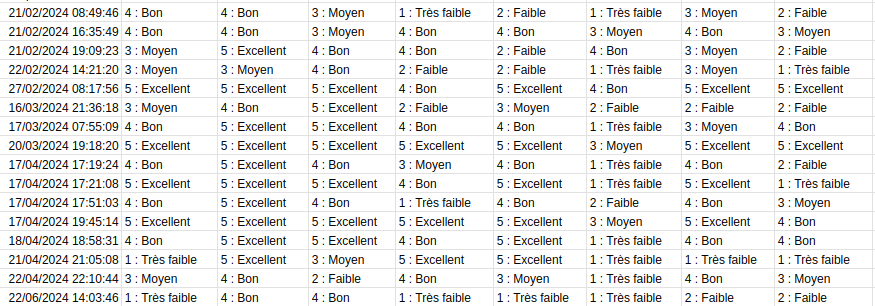
\includegraphics[width=15cm]{gfx/fig-eval.png}
    \caption{Extrait des évaluations reçues via Google Form}
    \label{fig:eval-result}
\end{figure}

\begin{figure}[H]
    \centering
    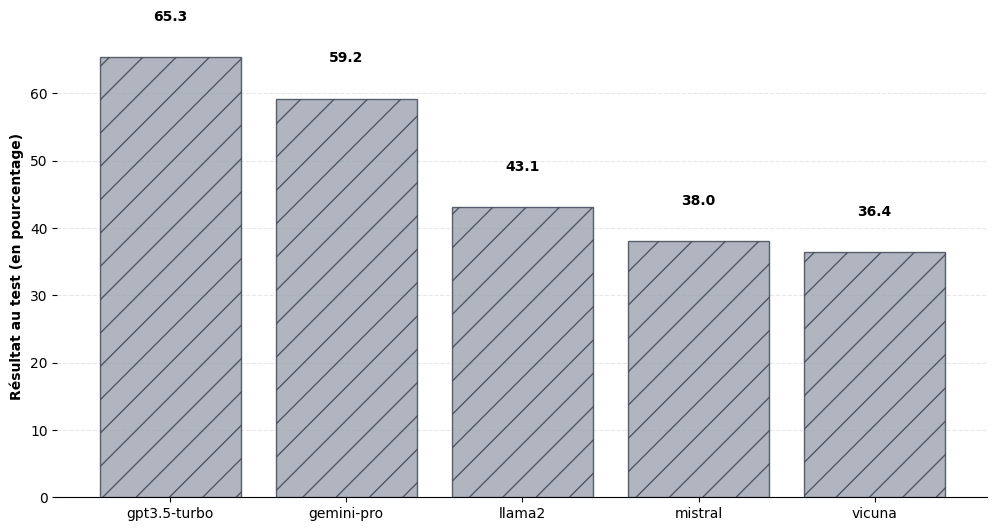
\includegraphics[width=15cm]{gfx/fig-model-result.png}
    \caption{Résultats après évaluation des différents modèles ,en pourcentage. (voir Code~\ref{appendix:code:python:model-result})}
    \label{fig:model-result}
\end{figure}

\newpage
\subsection{Évaluation quantitative}
Données de l'évaluation obtenues avec l'outil \href{https://artificialanalysis.ai/models/gemini-pro/prompt-options/single/medium}{artificialanalysis.ai}

\begin{figure}[H]
    \centering
    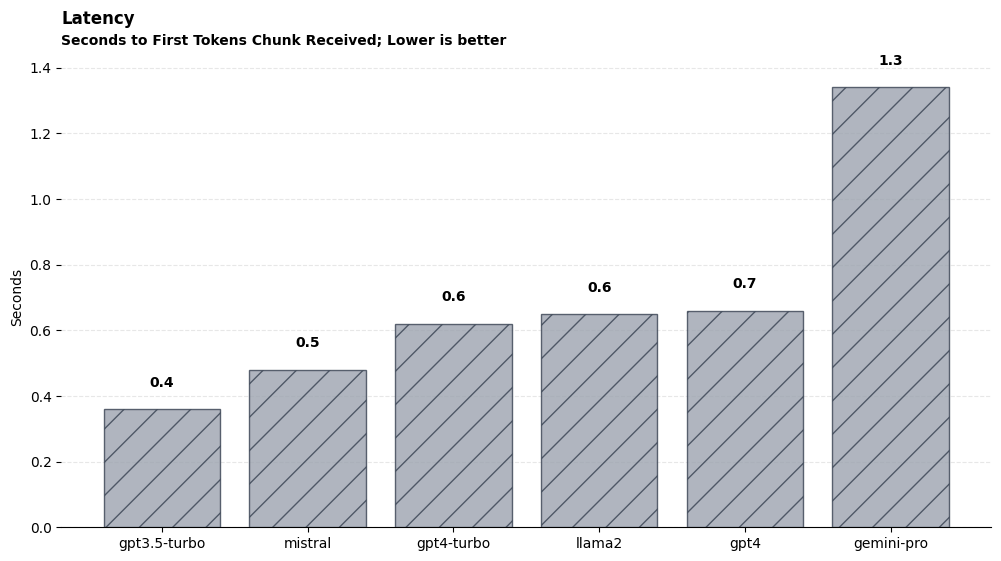
\includegraphics[width=15cm]{gfx/fig-latency-eval.png}
    \caption{Délai de réception du premier token, en secondes, après l'envoi de la demande d'\ac{api}.}
    \label{fig:model-latency-eval}
\end{figure}

\begin{figure}[H]
    \centering
    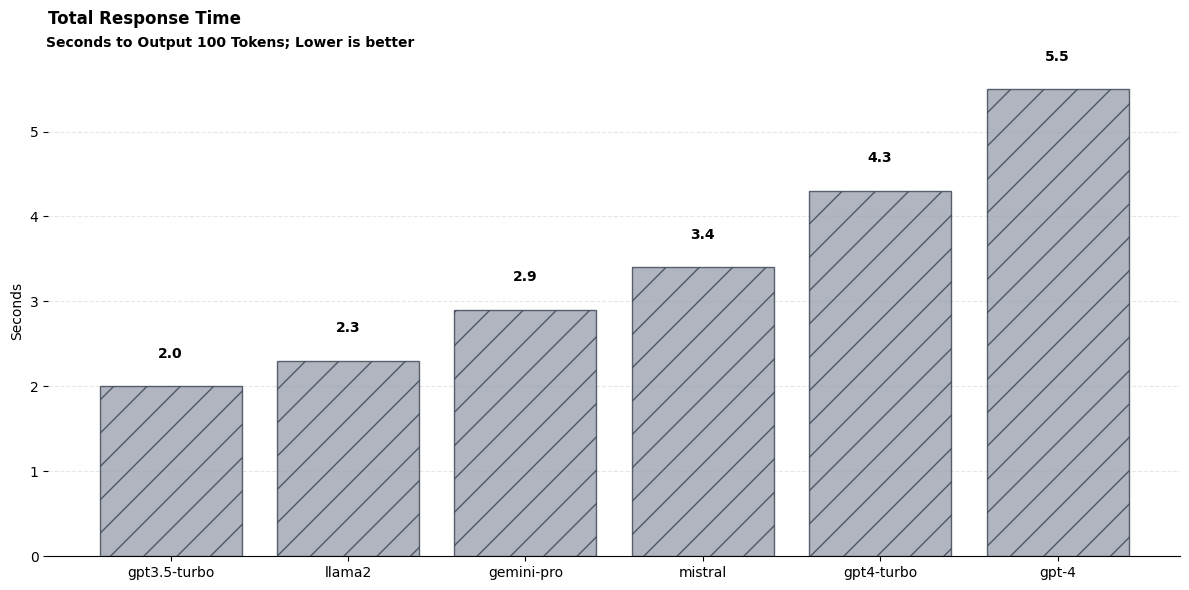
\includegraphics[width=15cm]{gfx/fig-response-time-eval.png}
    \caption{Temps nécessaire pour recevoir une réponse de 100 tokens. Estimation basée sur la latence (temps de réception du premier morceau) et la vitesse de sortie (nombre de tokens par seconde).}
    \label{fig:model-response-time-eval}
\end{figure}

\begin{figure}[H]
    \centering
    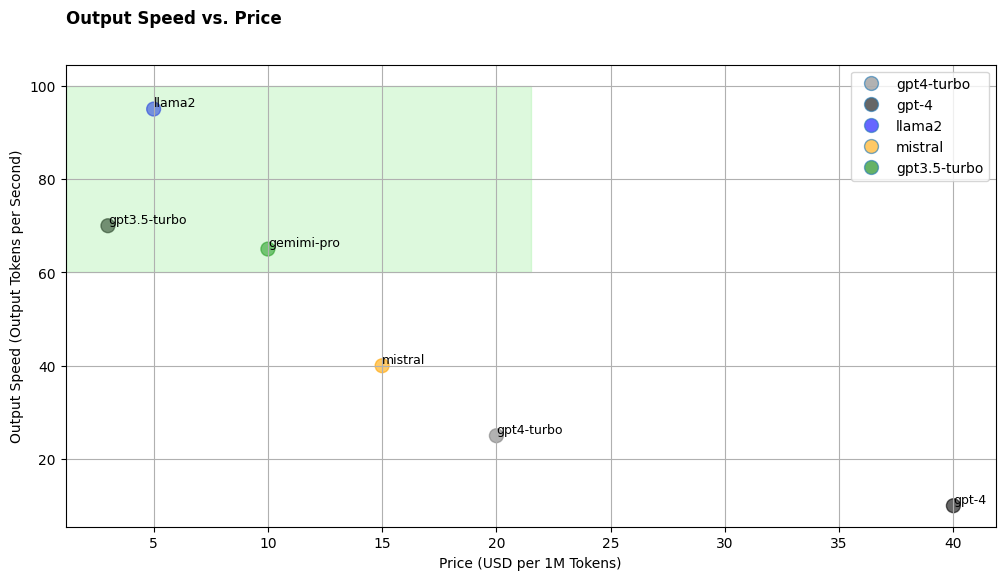
\includegraphics[width=15cm]{gfx/fig-price-speed-eval.png}
    \caption{Prix par token, représenté en USD par million de jetons. Le prix est un mélange des prix des tokens d'entrée et de sortie (ratio 3\:1).}
    \label{fig:model-price-speed-eval}
\end{figure}

L'évaluation quantitative révèle que les modèles d'entreprise, avec leurs ressources dédiées, garantissent une haute disponibilité. Cependant, au-delà des capacités intrinsèques de chaque modèle, l'infrastructure sous-jacente joue un rôle crucial dans les performances globales. 

Une infrastructure optimisée permet non seulement de maximiser l'efficacité des modèles, mais aussi d'assurer une réactivité et une fiabilité supérieures. La performance n'est donc pas uniquement liée à la sophistication du modèle, mais aussi à la robustesse et à l'efficacité de l'environnement dans lequel il opère. L'optimisation des serveurs, la gestion efficace des ressources et la minimisation des latences réseau sont autant de facteurs déterminants pour atteindre des performances de pointe.

\newpage
\newpage
\section{Évaluation de notre modèle}

Avant de procéder à une évaluation humaine, il est crucial de souligner la capacité de notre modèle à citer les sources utilisées pour générer ses réponses. 

\begin{figure}[H]
    \centering
    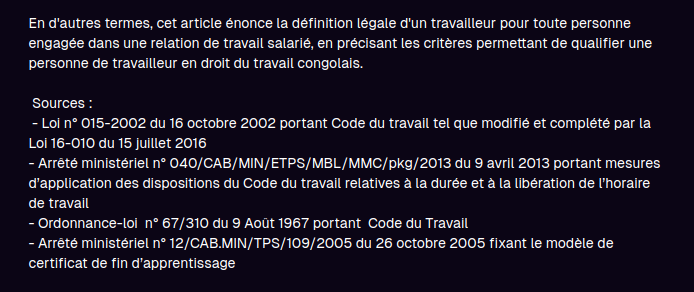
\includegraphics[width=15cm]{gfx/juro-source.png}
    \caption{Juro : Réponse avec citation}
    \label{fig:juro-source-citing}
\end{figure}

En citant les sources, notre modèle permet aux utilisateurs de vérifier l'origine des informations fournies, augmentant ainsi la confiance dans la validité et l'authenticité des réponses. Aussi la capacité à référencer les sources permet à notre modèle de mieux contextualiser les informations. Les utilisateurs peuvent comprendre non seulement le contenu de la réponse, mais aussi le contexte dans lequel cette information a été obtenue, enrichissant ainsi leur compréhension globale.

En fournissant des références, notre modèle aide les utilisateurs à approfondir leur recherche sur des sujets spécifiques. Ils peuvent consulter les sources originales pour obtenir des informations supplémentaires ou une perspective plus détaillée.

\subsection{Évaluation qualitative}

\begin{figure}[H]
    \centering
    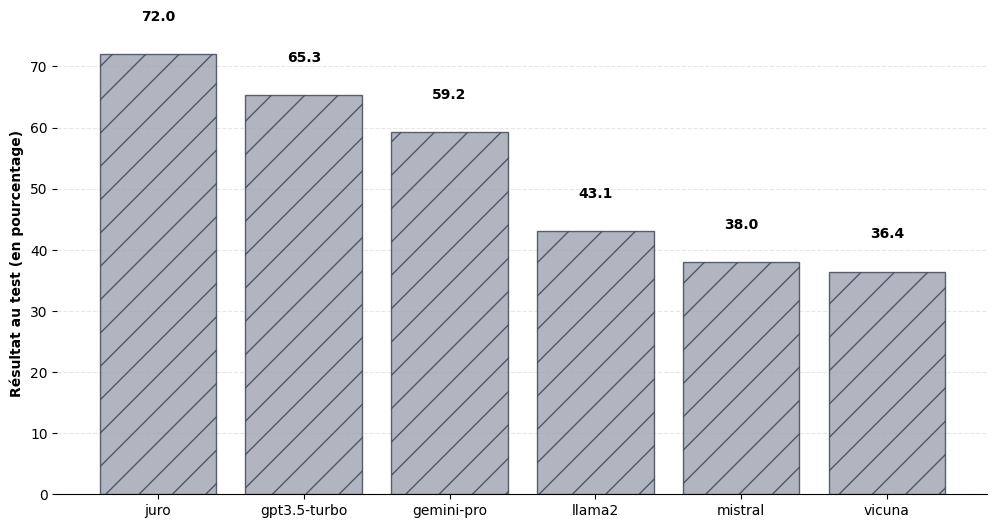
\includegraphics[width=15cm]{gfx/final-evaluation-juro.png}
    \caption{Résultats après évaluation de Juro par rapport aux modèles existants, en pourcentage.}
    \label{fig:final-evaluation-jur}
\end{figure}

Notre modèle Juro a également été évalué par des juristes, en utilisant le même procédé et la même méthodologie que pour les autres modèles. Cette évaluation a permis de mesurer la performance de Juro dans un contexte spécifique et pertinent, celui du droit congolais.

Les résultats finaux montrent que Juro surpasse significativement les autres modèles testés. Avec un score de 72\%, Juro se distingue par sa capacité à comprendre et à répondre aux questions juridiques congolaises de manière plus précise et plus pertinente. En comparaison, les autres modèles tels que GPT-3.5 Turbo (65.3\%), Gemini Pro (59.2\%), Llama2 (43.1\%), Mistral (38.0\%), et Vicuna (36.4\%) ont affiché des performances inférieures, soulignant ainsi l'avantage compétitif de Juro dans ce domaine.

\newpage
\subsection{Évaluation quantitative}

Pour évaluer quantitativement les performances de notre modèle, nous l'avons déployé sur une infrastructure cloud AWS (voir Section~\ref{ch:2:section:deploy}). Plus précisément, notre modèle a été hébergé sur une machine virtuelle avec les caractéristiques suivantes \textbf{2 GB RAM, 2 vCPUs, 60 GB SSD}. Cette configuration de base permet de mesurer la performance brute de notre modèle dans un environnement réaliste et accessible.

\begin{figure}[H]
    \centering
    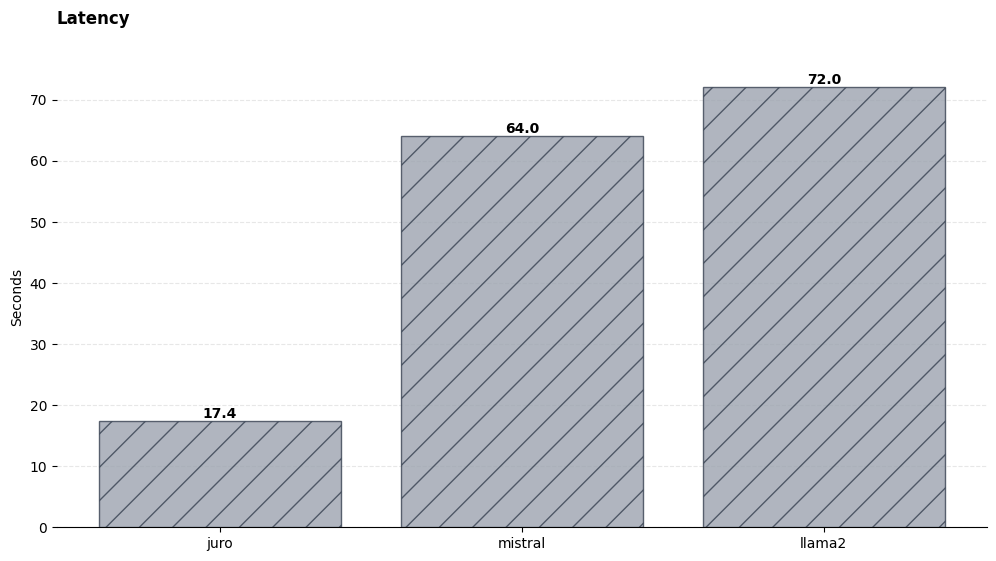
\includegraphics[width=15cm]{gfx/fig-latency-juro.png}
    \caption{Temps moyen nécessaire pour recevoir une réponse.}
    \label{fig:latency-juro}
\end{figure}

Pour notre modèle, nous nous appuyons sur les API de Mistral et OpenAI, ainsi que sur Ollama pour les modèles open source, notamment Mistral-7b et Llama-7b. L'inférence de ces modèles open source se fait sur notre propre serveur, qui gère également la récupération des documents nécessaires. Étant donné les spécifications techniques de notre serveur, le temps de réponse est naturellement plus lent, que ce soit pour les questions simples de droit, comme la recherche de lois, ou pour les questions doctrinales qui nécessitent un raisonnement approfondi. Cette lenteur inhérente à notre infrastructure impacte la rapidité de traitement et peut représenter un défi lors de l'interrogation de notre modèle pour des analyses juridiques complexes.

\newpage
\section{Résultats et perspectives}

Les évaluations qualitatives et quantitatives menées sur notre modèle montrent des résultats prometteurs mais également des pistes d'amélioration. Les principaux résultats obtenus sont :

\begin{enumerate}
    \item Les réponses générées par notre modèle se sont révélées globalement pertinentes et précises dans le contexte juridique. Cependant, certaines réponses nécessitent une compréhension plus approfondie des nuances juridiques et contextuelles.
    \item Les évaluations qualitatives via Google Form ont montré que les utilisateurs ont trouvé les réponses utiles mais ont parfois relevé des incohérences mineures.
    \item Le délai de réception du premier token après l'envoi de la demande d'API a été mesuré en secondes, révélant une latence plus élevée par rapport aux modèles d'entreprise. Cette différence est en grande partie due à notre infrastructure serveur moins optimisée.
    \item Le temps nécessaire pour recevoir une réponse de 100 tokens a également été mesuré, avec des résultats indiquant que la vitesse de sortie (nombre de tokens par seconde) pourrait être améliorée pour une meilleure réactivité.
\end{enumerate}

Les résultats obtenus ouvrent plusieurs voies d'amélioration et de développement futur :

\begin{enumerate}
    \item L'optimisation de l'infrastructure serveur pourrait réduire la latence et améliorer la réactivité globale du modèle. L'intégration de serveurs plus puissants et de technologies de mise à l'échelle automatique pourrait être envisagée.
    \item L'intégration de données spécifiques au domaine juridique et l'enrichissement continu du dataset utilisé pourraient améliorer la précision et la pertinence des réponses. Il est crucial de maintenir un dataset à jour et diversifié pour couvrir une large gamme de cas juridiques.
    \item La mise en place de fonctionnalités avancées telles que la compréhension contextuelle améliorée, la gestion des biais dans les données et la capacité à fournir des explications détaillées des réponses pourrait renforcer la confiance des utilisateurs et améliorer l'utilité du modèle.
    \item Encourager les collaborations entre experts en droit, ingénieurs en intelligence artificielle et autres parties prenantes est essentiel pour développer des solutions véritablement innovantes et adaptées aux besoins réels du secteur juridique. Les ateliers, les conférences et les projets communs pourraient favoriser l'échange de connaissances et de bonnes pratiques.
\end{enumerate}

En définitive, bien que notre modèle ait montré des résultats prometteurs, il reste encore beaucoup de travail à accomplir pour améliorer ses performances et répondre pleinement aux besoins du secteur juridique. Les perspectives d'avenir sont nombreuses et offrent de nombreuses opportunités pour exploiter le potentiel des technologies d'intelligence artificielle dans le domaine du droit.
